% DEVELOPMENT RUN --- not reportable; never include in the thesis.
% Generated by tools/pipeline/figures.py from a1_dryrun_20261009/metrics.json (sha256 9f27c701b18927a13a766588b5e230e6609dee023309588e844db05c92475d5a). Do not edit by hand.
\begin{figure}[htbp]
\centering
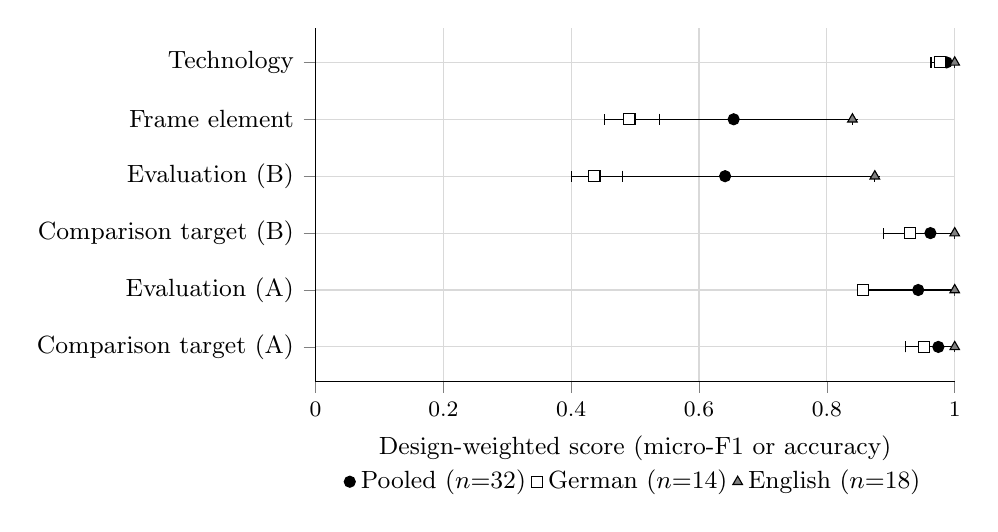
\begin{tikzpicture}
\begin{axis}[
  width=0.8\textwidth, height=0.5\textwidth,
  xmin=0, xmax=1, xlabel={Design-weighted score (micro-F1 or accuracy)}, xlabel style={font=\small},
  symbolic y coords={{Technology},{Frame element},{Evaluation (B)},{Comparison target (B)},{Evaluation (A)},{Comparison target (A)}}, ytick=data, y dir=reverse,
  yticklabel style={font=\small}, xticklabel style={font=\footnotesize},
  legend style={at={(0.5,-0.22)}, anchor=north, legend columns=3, font=\small, draw=none, fill=none},
  legend cell align=left, axis lines*=left, tick align=outside,
  enlarge y limits=0.12, grid=major, grid style={black!15},
]
\addplot[only marks, mark=*, mark options={fill=black, draw=black}, error bars/.cd, x dir=both, x explicit] coordinates {(0.9873,{Technology}) -= (0.0244,0) += (0.0127,0) (0.6542,{Frame element}) -= (0.2026,0) += (0.1858,0) (0.6408,{Evaluation (B)}) -= (0.2408,0) += (0.2342,0) (0.9620,{Comparison target (B)}) -= (0.0731,0) += (0.0380,0) (0.9429,{Evaluation (A)}) -= (0.0857,0) += (0.0571,0) (0.9744,{Comparison target (A)}) -= (0.0513,0) += (0.0256,0)};
\addplot[only marks, mark=square*, mark options={fill=white, draw=black}, error bars/.cd, x dir=both, x explicit] coordinates {(0.9767,{Technology}) -= (0.0138,0) += (0.0233,0) (0.4912,{Frame element}) -= (0.0396,0) += (0.0472,0) (0.4364,{Evaluation (B)}) -= (0.0364,0) += (0.0436,0) (0.9302,{Comparison target (B)}) -= (0.0413,0) += (0.0698,0) (0.8571,{Evaluation (A)}) -= (0.0000,0) += (0.0000,0) (0.9524,{Comparison target (A)}) -= (0.0293,0) += (0.0476,0)};
\addplot[only marks, mark=triangle*, mark options={fill=black!50, draw=black}, error bars/.cd, x dir=both, x explicit] coordinates {(1.0000,{Technology}) -= (0.0000,0) += (0.0000,0) (0.8400,{Frame element}) -= (0.0000,0) += (0.0000,0) (0.8750,{Evaluation (B)}) -= (0.0000,0) += (0.0000,0) (1.0000,{Comparison target (B)}) -= (0.0000,0) += (0.0000,0) (1.0000,{Evaluation (A)}) -= (0.0000,0) += (0.0000,0) (1.0000,{Comparison target (A)}) -= (0.0000,0) += (0.0000,0)};
\legend{{Pooled ($n$=32)},{German ($n$=14)},{English ($n$=18)}}
\end{axis}
\end{tikzpicture}
\caption{\textbf{DEVELOPMENT RUN --- not reportable.} Headline agreement between the model's first execution and the human reference, by scoring dimension and population. Marks are design-weighted point estimates; bars are the 2.5--97.5 percentile interval over 2000 article resamples. Run \texttt{a1\_dryrun\_20261009}.}
\label{fig:primary}
\end{figure}
